\chapter{Methodik und Implementierung}\label{ch:MethodikUndImplementierung}
Dieses Kapitel führt das Vorgehen und die Implementierung eines C++ Programms aus.
Dadurch wird es möglich, Aussagen über den Speicher des Kaffeevollautomaten zu treffen.
Immer wiederkehrende Arbeitsabläufe werden von diesem Programm übernommen und auf den unteren Ebenen automatisiert.

\section{Vorgehen}\label{sec:Vorgehen}
Die Speicher des Kaffeevollautomaten, der \ac{EEPROM} und der \ac{RAM}, können zeilenweise ausgelesen werden.
Der nötige Zugriff zum Auslesen kann auf zwei Arten erfolgen: direkt am Speicherstein auf der Hauptplatine oder seriell über die vorhandene \ac{UART} Schnittstelle.
Abschnitt~\ref{subsec:zugangSeriellDirekt} diskutiert die Vor- und Nachteile, die dazu geführt haben im Folgenden die Kommunikation über die \ac{UART} Schnittstelle und mithilfe der \textit{libserial}-Library erfolgen zu lassen.
Dadurch kann die Speicherabfrage als Blackbox Modell, ähnlich zum Blackbox Testing in \cite{Solr-599853700}, betrachtet werden, wo nur mit Ein- und Ausgaben des Kaffeevollautomaten gearbeitet wird, ohne dessen Programm zu kennen.

Unabhängig voneinander wurden beide Speicher untersucht.
Ein eigens entwickeltes C++ Programm setzt die 16 Zeilen einer Speicherabfrage zu einem gesamten Speicherauszug zusammen.
Intern werden dabei je zwei Hexadezimalzahlen in eine ganzzahlige Dezimalzahl umgerechnet und in einem Vektor abgelegt.
Dadurch sind Position und Wert bekannt.

\begin{figure}
  \begin{center}
    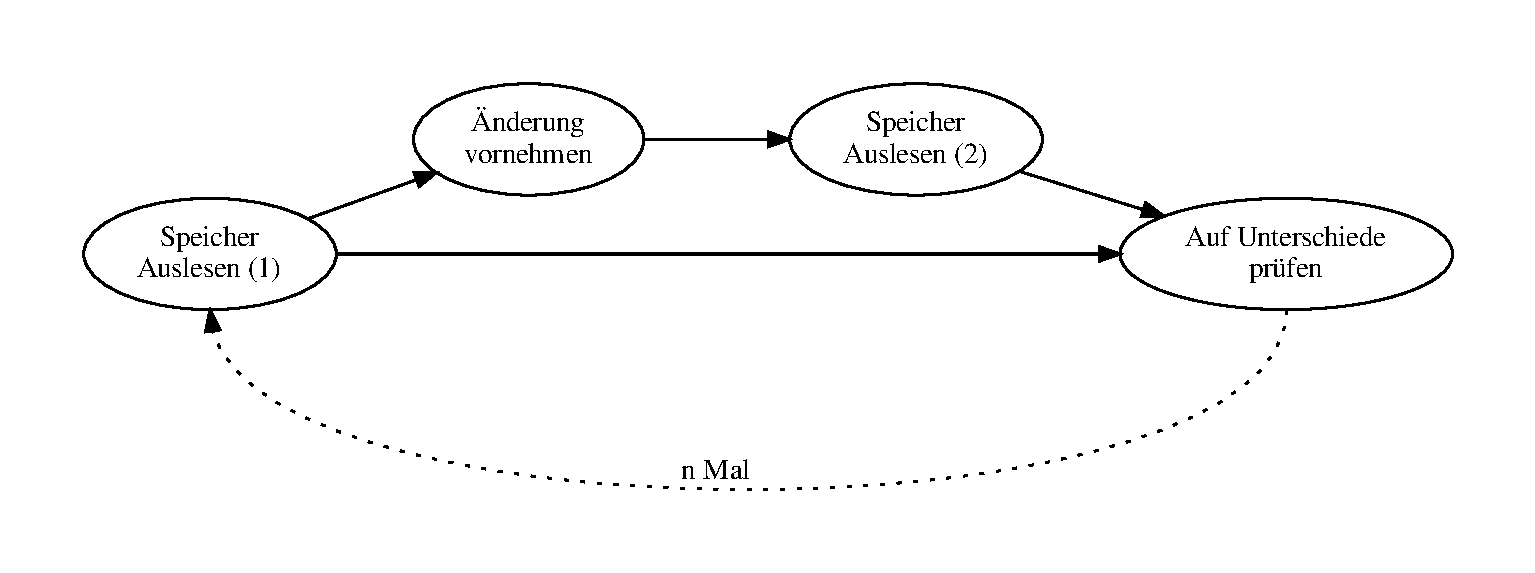
\includegraphics[scale=0.6]{images/chapter_4/workflow}
    \caption{Arbeitsablauf zur systematischen Untersuchung des EEPROMs und RAMs}
    \label{fig:workflow}
  \end{center}
\end{figure}

Abbildung~\ref{fig:workflow} visualisiert den Arbeitsablauf, der zur Bestimmung der Speicherstellen in dieser Arbeit angewandt wurde.
Nach dem ersten Schritt ganz links wird nun von Hand eine möglichst elementare Veränderung an dem Kaffeevollautomaten vorgenommen, um gezielten Aktionen die Werteänderungen bestimmter Speicherzellen zuordnen zu können.
Die angewandten Veränderungen werden in Abschnitt~\ref{subsec:AenderungenAnDerMaschine} beschrieben.

Nach einer erneuten Aufnahme eines Speicherauszugs können diese beiden nun verglichen werden.
Das Programm iteriert durch den Vektor und vergleicht die Speicherwerte an der gleichen Position.
Bei Ungleichheit existiert ein Unterschied, der festgehalten wird.
Dieser Ablauf wurde auf alle Einstellmöglichkeiten und Funktionen des Kaffeevollautomaten angewandt.

Bei dem \ac{RAM}, im Gegensatz zum \ac{EEPROM}, fiel jedoch auf, dass sich mehrere Speicherwerte auch ohne eine vorgenommene Veränderung änderten.
Deshalb wurden viele Speicherauszüge im Ruhezustand aufgenommen und die sich regelmäßig ändernden Bytes ausgeschlossen.
Zu Beginn der Ergebnisse über den \ac{RAM} in Abschnitt~\ref{sec:ErgebnisseRAM} sind diese aufgeführt.
Dennoch gab es gelegentliche Unregelmäßigkeiten, sodass das Vorgehen für den \ac{RAM} um eine geschlossene Rückrichtung ergänzt wurde.
In der Regel wurden pro \ac{RAM} Funktion $n=3$ Durchläufe vorgenommen und die gemeinsame Schnittmenge der Veränderungen bestimmt.

Bei einem zweiten Vorgehen wurde gezielt der \ac{EEPROM} an bekannten Speicherstellen beschrieben.
Hintergrund war die unbekannte Position bzw. später die Zusammensetzung des Bezüge-Zählers im Einstellungsmenü des Kaffeevollautomaten.
Abschnitt~\ref{subsec:Vorgehen2} führt dies im Folgenden aus.

\subsection{Veränderungen zur Bestimmung der Speicherstellen}\label{subsec:AenderungenAnDerMaschine}
\subfigbox{
  \subfigure[Dargestellt ist die Fassung im Kaffeevollautomaten.]{\label{subfig:fassung}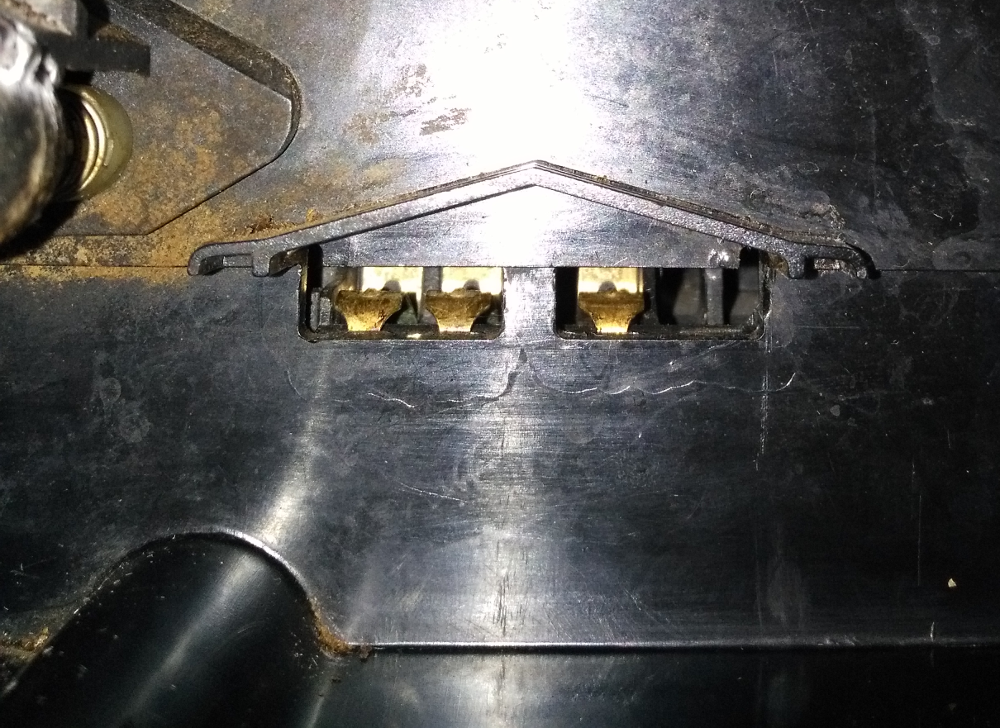
\includegraphics[scale=0.2]{images/chapter_4/Schale-Fassung}}\\%
  \subfigure[Zu sehen ist die Oberseite des Ersatzes für die Schale.]{\label{subfig:oberseite}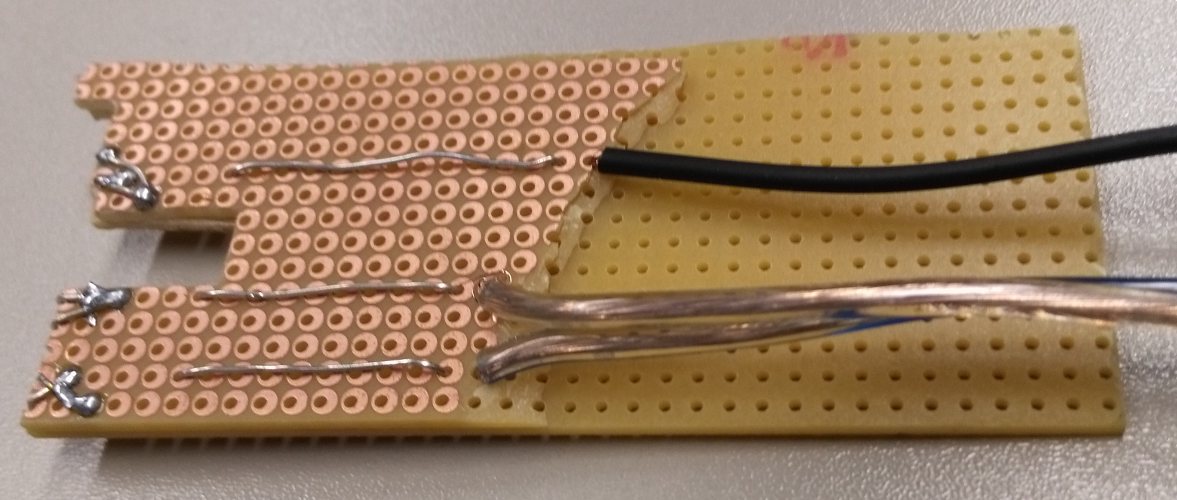
\includegraphics[scale=0.29]{images/chapter_4/Schale-Oberseite}}\\%
  \subfigure[Zu sehen ist die Unterseite des Ersatzes für die Schale.]{\label{subfig:unterseite}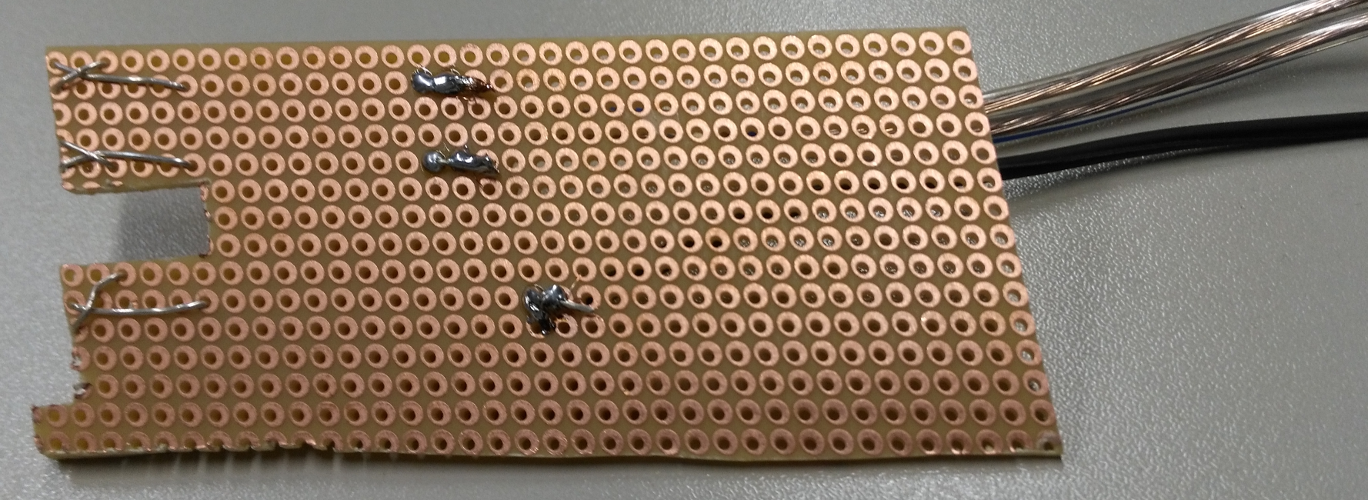
\includegraphics[scale=0.25]{images/chapter_4/Schale-Unterseite}}%
}{Ersatz der Schale des Kaffeevollautomaten}{fig:ersatzschale}

Für den \ac{EEPROM} war es hilfreich, systematisch durch das Handbuch der Maschine zu gehen und zum Beispiel immer eine Menüoption zu variieren.
Bei einer Skala (wie z.B. beim Kaffeepulver) hat es ausgereicht, den niedrigsten, den höchsten und den Standard-Wert im Speicher zu bestimmen;
deckte sich die einstellbare Anzahl an Abstufungen mit der Differenz der Werte im Speicher, ließ sich auf die verbleibenden Werte schließen.
Auch im normalen Gebrauch fiel unter anderem ein Einschaltzähler im \ac{EEPROM} auf.

Für den \ac{RAM} ging es mit den gezielt auslösbaren Statusmeldungen los.
Das Anheben des Wassertanks oder das Abziehen der unteren Schale löste eine Warnmeldung auf dem Display aus und wurde auch im \ac{RAM} vermerkt.
Ein zu hoher Wasserstand in der Schale konnte ohne Wasser mit einer eigenen Platine vorgegaukelt werden.
Abbildung~\ref{subfig:fassung} zeigt die Fassung an der Rückwand innerhalb des Kaffeevollautomaten für die Schale.
Abbildung~\ref{subfig:oberseite} und \ref{subfig:unterseite} visualisieren die Platine, an der leicht von außen mittels Krokodilklemmen die Kontakte im Inneren kurzgeschlossen werden konnten.
Am schwierigsten sind komplexe Abläufe, wie die Zubereitung eines Kaffees.
Hier konnte nur mehrfach zu gezielt gleichen oder ungleichen Zeitabständen der zweite Speicherauszug angestoßen werden.

Abschließend war auch für das Display ein kleines Programm nötig, um die volle Funktionsvielfalt festzustellen.
Abschnitt~\ref{subsec:tools} führt dies später aus.

In Abschnitt~\ref{sec:AussagekraftDerErgebnisse} wird die Aussagekraft dieser Ergebnisse noch thematisiert.

\subsection{EEPROM gezielt beschreiben}\label{subsec:Vorgehen2}
Ziel war es die unbekannte Position bzw. später die Zusammensetzung des Bezüge-Zählers im Einstellungsmenü des Kaffeevollautomaten zu entziffern.
Dafür wurde die angezeigt Zahl in eine Hexadezimalzahl umgerechnet und im Speicherauszug des \ac{EEPROM} des Kaffeevollautomaten gesucht.
Da die Zahl eine Stromunterbrechung überstand und eine Änderung des einzigen übereinstimmenden Wertependants in Wort \wort{15} keine Änderung der Ausgabe hervorrief, begann die Suche an weiteren bekannten Speicherstellen im \ac{EEPROM}.
Bekannte Zähler in Wörtern wie \wort{00}, \wort{01}, \wort{02}, \wort{0D}, \wort{0E} oder mehreren weiteren wurden einzeln auf sehr hohe Werte geändert.
Manche Änderungen veränderten den Bezüge-Zähler oder lösten Warnmeldungen an dem Kaffeevollautomaten aus.

Es folgte die Erkenntnis, dass sich der Bezüge-Zähler aus mehreren Zählern zusammen setzt.
Der Trester Füllstand in der Schale wird nicht gemessen, sondern im Betrieb gezählt, um den Füllstand zu erfassen.
Auch die Reinigungsankündigung beruht auf Zählerständen über Kaffeebezüge und Spülungen.
Die Wasser-Durchflussmenge des Filters wird ebenfalls erfasst und ab einem festen Wert eine Warnmeldung zum Wechseln ausgegeben.

Das gezielte Eingreifen in die Zählerstände ließ es zu, diese Grenzwerte exakt zu bestimmen.
Die Ergebnisse befinden sich in Abschnitt~\ref{subsec:ErgebnisKaffeezubereitung}.

\section{Das C++ Programm "`./JuraCoffeeMemory"'}
Für diese Arbeit wurde ein C++ Programm entwickelt, das die Kommunikation und die Aufschlüsselung der Antworten übernommen hat.

\subsection{Makefile}
In dem Projekt Ordner befinden sich auf der Hauptebene mehrere \texttt{CPP}- und \texttt{HPP}-, eine \texttt{H}- sowie eine \texttt{Makefile}-Datei.
Sind die in der \texttt{Readme.md} genannten Abhängigkeiten und Voraussetzungen erfüllt, kann das Projekt mit dem Befehl \texttt{make} ohne Zusatzangaben kompiliert werden.
Am Ende sollte dann auf der Hauptebene eine ausführbare Datei namens \texttt{./JuraCoffeeMemory} herauskommen.
Es werden neben Objekt-Dateien auch noch einige weitere Tools im Unterordner \texttt{./tools/} erstellt, auf die später in Abschnitt~\ref{subsec:tools} eingegangen wird.

Der Befehl \texttt{make clean} entfernt die Objekt-Dateien; mittels \texttt{make dist-clean} werden ebenfalls die ausführbaren Programme entfernt und der Projekt-Ordner wird in seinen Ursprungszustand zurück versetzt.

\subsection{Interaktives Menü}
Startet man in einem Terminal das Hauptprogramm \texttt{./JuraCoffeeMemory} wird das Hauptmenü angezeigt. Abbildung~\ref{subfig:terminal1-MainMenu} visualisiert diesen Zustand.
Das Listing~\ref{lst:menu-tree} zeigt schematisch alle Menüoptionen.

\subfigbox{
  \subfigure[Hauptmenü]{\label{subfig:terminal1-MainMenu}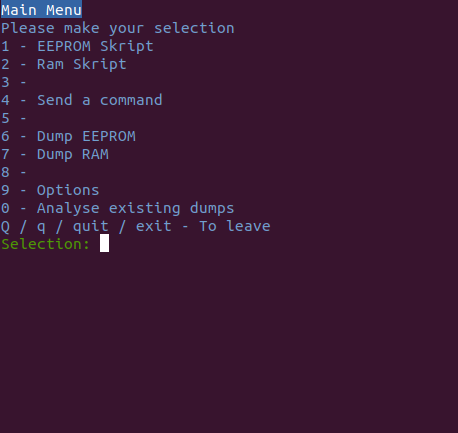
\includegraphics[scale=0.4]{images/chapter_4/JuraCoffeeMemory-1-MainMenu}}\hfill%
  \subfigure[EEPROM Skript]{\label{subfig:terminal3-EEPROM-NothingChanged}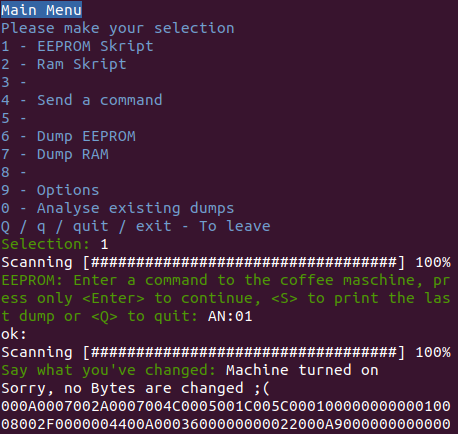
\includegraphics[scale=0.4]{images/chapter_4/JuraCoffeeMemory-3-EEPROM-NothingChanged}}\\%
  \subfigure[RAM Speicherauszug]{\label{subfig:terminal5-RAM-dump}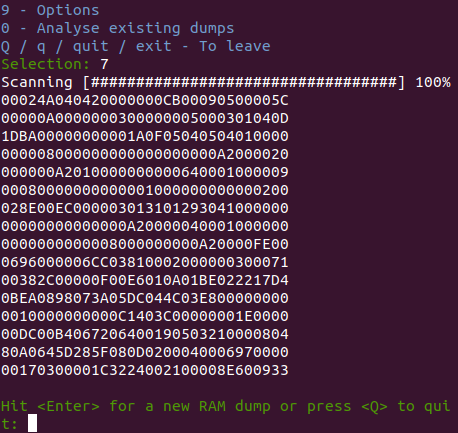
\includegraphics[scale=0.4]{images/chapter_4/JuraCoffeeMemory-5-RAM-dump}}\hfill%
  \subfigure[Optionen $\leadsto$ Log Pfad ändern]{\label{subfig:terminal7-Options-RamLogFilePath}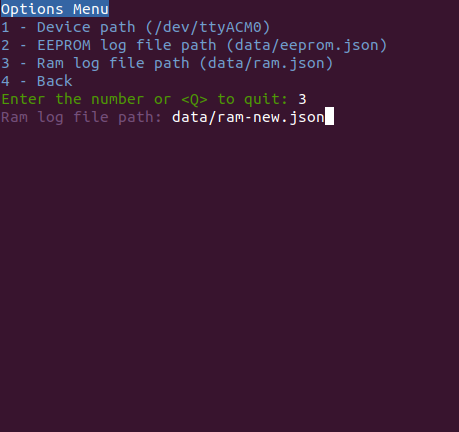
\includegraphics[scale=0.4]{images/chapter_4/JuraCoffeeMemory-7-Options-RamLogFilePath}}\\%
%  \subfigure[Befehl senden]{\label{subfig:terminal4-Send-TY}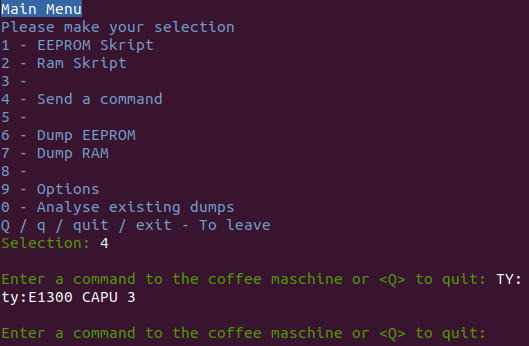
\includegraphics[scale=0.4]{images/chapter_4/JuraCoffeeMemory-4-Send-TY}}%
  \subfigure[Auswertungen]{\label{subfig:terminal8-AnalyseDumpsMenu}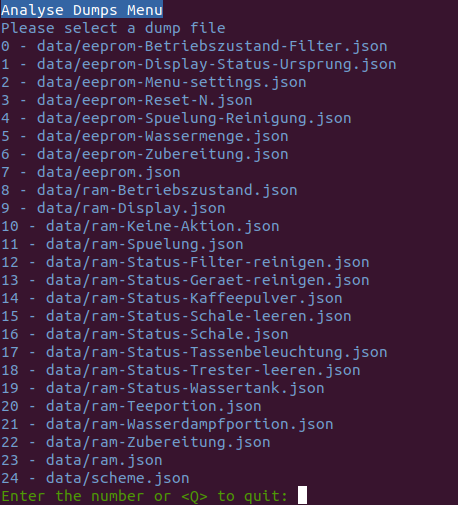
\includegraphics[scale=0.3]{images/chapter_4/JuraCoffeeMemory-8-AnalyseDumpsMenu}}\hfill%
  \subfigure[Speicherauszug einsehen]{\label{subfig:terminal9-AnalyseFilterDump}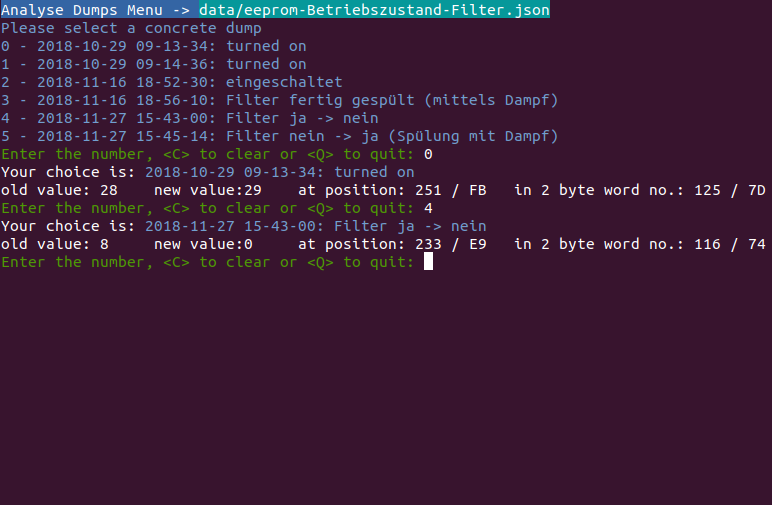
\includegraphics[scale=0.3]{images/chapter_4/JuraCoffeeMemory-9-AnalyseFilterDump}}%
}{Interaktives Menü des C++ Programms "`./JuraCoffeeMemory"'}{fig:terminal}

\begin{lstlisting}[label=lst:menu-tree,caption={Menü-Baum ./JuraCoffeeMemory}]
Main Menu
|-- 1: EEPROM Skript
|-- 2: Ram Skript
|-- 4: Send a command
|-- 6: Dump EEPROM
|-- 7: Dump RAM
|-- 9: Options
|   |-- 1: Device path (/dev/ttyACM0)
|   |-- 2: EEPROM log file path (data/eeprom.json)
|   |-- 3: Ram log file path (data/ram.json)
|   `-- 4: Back
|-- 0: Analyse existing dumps
|   |-- Analyse Dumps Menu
|   |   |-- data/xxx.json
|   |   |   `-- Dumps
|   |   |-- C: Clear window
|   |   `-- Q: Quit
|   `-- Q: Quit
`-- Q / q / quit / exit: To leave
\end{lstlisting}

\subsubsection{EEPROM / RAM Skript}\label{subsubsec:EEPROM-RAM-Skript}
Über die Nummer \texttt{1} startet aus dem Hauptmenü das \textit{EEPROM Skript}, über die \texttt{2} das \textit{RAM Skript}.
Siehe hierfür Abbildung~\ref{subfig:terminal3-EEPROM-NothingChanged}.
In beiden Fällen wird das Vorgehen in Abschnitt~\ref{sec:Vorgehen} angewendet.
Das Skript erzeugt initial einen Speicherauszug und merkt sich diesen.
Der Anwender kann sich diesen über die Eingabe \texttt{S} ausgeben lassen oder an diesem Punkt über \texttt{Q} das Skript beenden.
Um fortzufahren kann nun eine Aktion vorgenommen oder direkt ein Befehl abgesetzt werden.
Das Skript erstellt im Anschluss einen weiteren Speicherauszug und fragt nach einem Kommentar zu den vorgenommenen Änderungen.
Nach einer Texteingabe vergleicht das Programm die Speicherauszüge und hält Unterschiede in der Standardausgabe und der \ac{JSON} Ausgabedatei fest.
Ebenso werden in der \ac{JSON} Datei jedes Mal beide Speicherauszüge mit Zeitstempel und Kommentar abgelegt.
Das Skript verwirft den vorletzten Speicherauszug und bietet die Fortführung mit dem Anwender Menü an.

\subsubsection{Einen Befehl abschicken}
Über die Nummer \texttt{4} startet aus dem Hauptmenü eine immer wiederkehrende Eingabeaufforderung, in der Befehle aus der Tabelle~\ref{tbl:kommandos} an den Kaffeevollautomaten verschickt werden können.
Hierüber kann schnell ein Funktionstest der Verbindung zum Kaffeevollautomaten vorgenommen werden.
Über \texttt{Q} kehrt der Anwender in das Hauptmenü zurück.

\subsubsection{Speicherauszug}
Über die Nummer \texttt{6} bzw. Nummer \texttt{7} kann ein einzelner Speicherauszug des \ac{EEPROM}s bzw. des \ac{RAM}s erstellt werden, der unverzüglich in der Standardausgabe ausgegeben wird.
Abbildung~\ref{subfig:terminal5-RAM-dump} zeigt einen Speicherauszug des \ac{RAM}s.
Diese Funktion ist ein Teil des \ac{EEPROM} bzw. \ac{RAM} Skripts.
Es fragt aber nicht nach einem Kommentar und fungiert an dieser Stelle rein lesend.
Mithilfe des Hilfsprogramms zum Formatieren eines Speicherauszugs aus Abschnitt~\ref{subsec:formate-dump} kann man den Speicherauszug um Positionsangaben aufwerten und Speicherwerte dadurch kontrollieren.

\subsubsection{Optionen}
Über die Nummer \texttt{9} gelangt der Anwender in das Optionsmenü, wie in Abbildung~\ref{subfig:terminal7-Options-RamLogFilePath} dargestellt.
Es können für den aktuellen Prozess der Pfad zum Gerätelaufwerk des Arduinos und die Ausgabedateien für das \ac{EEPROM} und \ac{RAM} Skript angepasst werden.
Nach der Eingabe eines neuen Pfades wird dieser sofort übernommen und angezeigt.
Über die Nummer \texttt{4} kehrt der Anwender in das Hauptmenü zurück.

\subsubsection{Analyse aufgenommener Speicherauszüge}
In der \ac{JSON} Datei werden im Knoten \texttt{"data"} die Wertänderungen hinter jedem entsprechenden Byte inklusive Kommentar festgehalten.
Nach mehreren Durchläufen des \ac{EEPROM} / \ac{RAM} Skripts können hier schon direkt einige Zugehörigkeiten abgelesen werden.

Das C++ Programm bietet über die Nummer \texttt{0} auch die Option Unterschiede einzelner Aufnahmen über das Skript erneut auszugeben.
Zuerst werden sämtliche \ac{JSON} Dateien im Unterordner \texttt{data/} aufgelistet, siehe Abbildung~\ref{subfig:terminal8-AnalyseDumpsMenu}.
Nach der Wahl einer Datei wird eine Übersicht aller darin enthaltener Speicherauszüge ausgegeben.
Durch die Wahl der entsprechenden Nummer werden der Kommentar und die veränderten Werte pro Byte aufgeschlüsselt.
In Abbildung~\ref{subfig:terminal9-AnalyseFilterDump} ist dies für zwei Speicherauszüge dargestellt, die jeweils nur eine Änderung beinhalten.

\subsubsection{Angaben in der Aufschlüsselung der Veränderungen}
Sowohl im \ac{EEPROM} / \ac{RAM} Skript als auch in der Analyse aufgenommener Speicherauszüge können Veränderungen eingesehen werden.
Das erste Beispiel aus Abbildung~\ref{subfig:terminal9-AnalyseFilterDump} lautet:
\begin{lstlisting}[label=lst:dumpChanges,caption={Beispiel einer Abweichung zweier Speicherauszüge}]
Your choice is: 2018-10-29 09-13-34: turned on
old value: 28  new value:29  at position: 251 / FB  in 2 byte word no.: 125 / 7D
\end{lstlisting}
Diese Ausgabe ist für den \ac{EEPROM} und \ac{RAM} prinzipiell gleich, die relevanten Stellen sind aber leicht verschieden.
Zu Beginn erscheint die Uhrzeit und der bei der Aufnahme eingegebene Kommentar.
Pro Zeile folgt danach eine Änderung.
In diesem Fall änderte sich der Wert von \texttt{28} auf \texttt{29}.
Diese Aufnahme kommt aus dem \ac{EEPROM}, für den die Befehle auf den 2 Byte \textit{Wort} Adressen beruhen.
Möchte man diesen Wert verändern, ist die letzte Spalte mit der hexadezimalen Zahl von Bedeutung, zum Beispiel \texttt{WE:7D,xxxx}.

Für den \ac{RAM} ist die normale Position eines Bytes von Bedeutung, hier würde sich der dezimale Wert \texttt{29} an der Position \texttt{FB} befinden.
Über den Befehl \texttt{RR:FB} bekäme man die \texttt{29} als anfängliche Hexadezimalzahl zurück gegeben.

\subsubsection{Farbcodierungen}
Die verwendeten Farben sollen dem Anwender Orientierung und Struktur bei der Benutzung verschaffen.
Normale Ausgaben und Benutzereingaben erscheinen in weißer Schrift.
Weiße Schrift auf blauem Grund stellt Menü-Überschriften dar.
In blauer Schrift sind Menüs dargestellt.
Grüne Schrift vor der blinkenden Eingabemarke fordert zur Eingabe auf.
Der Text beschreibt valide Eingaben.
Abschließend beschreibt roter Text einen Fehler.
Die aufgetretene Position wird in weißer Schrift auf rotem Grund hervorgehoben.

\subsection{Die API nach außen}
Das Hauptprogramm kann auch über vier Parameter aufgerufen werden. Die Ausgaben sind dann im fehlerfreien Fall farblose \ac{JSON} Zeichenketten oder einfacher Text in die Standardausgabe.

Mögliche Fehlermeldungen sind für Entwickler in der \texttt{Readme.md} dokumentiert.
Die Fehlerausgabe erfolgt wie im interaktiven Menü mit Farben.
Für Entwickler bietet sich daher der Rückgabewert des Programms an.

\paragraph{./JuraCoffeeMemory command}
Von der Standardeingabe wird eine Zeichenkette erwartet, die an den Kaffeevollautomaten weiter gegeben wird.
Mögliche Eingaben sind die Befehle aus der Tabelle~\ref{tbl:kommandos}.
Die Antwort des Kaffeevollautomaten erscheint als einfacher Text.

\paragraph{./JuraCoffeeMemory eepromWrite}
Bei diesem Aufruf wird von der Standardeingabe ein \ac{JSON} Objekt erwartet.
Alle dort genannten Bezeichnungen werden abgearbeitet und die neuen Werte im Speicher des Kaffeevollautomaten hinterlegt.
Auf der obersten Ebene müssen sich aus \texttt{EEPROM\_Status::getEntriesEEPROM()} bekannte Bezeichnungen befinden, die ein Unterobjekt mit der Bezeichnung \texttt{value} sowie je einen ganzzahligen Wert beinhalten.
Listing~\ref{lst:eepromWrite} veranschaulicht dies an einem Beispiel.

Treffen die Bedingungen zu, wird ein Schreib-Befehl an den Kaffeevollautomaten gesandt.
Die Antworten werden in einer Zeichenkette mit der verwendeten Bezeichnung und dem Text "`\#\#\#"' als Abstandshalter festgehalten und auf der Standardausgabe ausgegeben.
Die Antwort auf das Beispiel Listing~\ref{lst:eepromWrite} steht in Listing~\ref{lst:eepromWriteAnswer}.

\begin{lstlisting}[label=lst:eepromWrite,caption={Beispiel einer JSON Eingabe für./JuraCoffeeMemory eepromWrite}]
{
  "powder_quantity_special_coffee": {
    "value": 11
  },
  "water_quantity_special_coffee": {
    "value":  380
  }
}
\end{lstlisting}

\begin{lstlisting}[label=lst:eepromWriteAnswer,caption={Antwort auf das Beispiel der JSON Eingabe}]
ok: powder_quantity_special_coffee###ok: water_quantity_special_coffee###
\end{lstlisting}

\paragraph{./JuraCoffeeMemory eeprom}
Nach ungefähr 5 Sekunden erhält man die aktuellen Einstellungen und Zählerstände des \ac{EEPROM} in einem kompakten \ac{JSON} Objekt.
Im Gegensatz zum EEPROM Skript werden nur die nötigen Speicherstellen abgefragt.
Die Bezeichnung der Speicherstellen, die auch der Name eines \ac{JSON} Eintrags ist, befindet sich mit der zugehörigen Adresse in \texttt{EEPROM\_Status::getEntriesEEPROM()}.
Eine Adresse besteht aus der Position eines Wortes sowie einer oder beiden Bytes.
Von Hand sind dort zum Teil weitere Hintergrundinformationen, wie Standardwerte über die \texttt{[N]}-Taste des Kaffeevollautomaten, minimale und maximale Schranken, der Wert für einen deaktivierten Zustand oder überhaupt zulässige Werte, hinterlegt.

\paragraph{./JuraCoffeeMemory ram}
Ähnlich zum Abfragen des \ac{EEPROM} wird hier aber der \ac{RAM} in ungefähr 3 Sekunden an den entscheidenden Stellen ausgelesen.
Die Assoziation einer Bezeichnung mit ihrer Speicherposition geschieht in \texttt{RAM\_Status::getEntriesRAM()}.
Hier wird ein Byte und ggf. mehrere zusammenhängende Bits als ein Eintrag abgelegt.
Als Ausgabe erfolgt ein kompaktes \ac{JSON} Objekt.

\subsection{Technische Umsetzung}
Abbildung~\ref{fig:storage_inherit_graph} zeigt schematisch den Zusammenhang der C++ Klassen.
Die Hauptdatei ist die \texttt{JuraCoffeeMemory.cpp}, aus der später auch das ausführbare Programm \texttt{./JuraCoffeeMemory} erzeugt wird.
Sie steht ganz oben in Abbildung~\ref{fig:storage_inherit_graph}.
Die \texttt{main}-Funktion fängt die Argumente des Programm-Aufrufs ab und übergibt entsprechend an die \texttt{EEPROM\_Status} bzw. \texttt{RAM\_Status} Klasse für die \ac{API} oder leitet den Anwender selber durch das interaktive Menü.
Die \textit{API}-Box in Abbildung~\ref{fig:storage_inherit_graph} repräsentiert die \ac{API} mit den beiden Klassen.

Beim Aufruf des \ac{EEPROM} Skripts wird die \texttt{eeprom}-Funktion betreten, für den \ac{RAM} analog die \texttt{ram}-Funktion.
Diese Funktionen bauen zu Beginn eine serielle Verbindung zum Arduino auf und blockieren damit alle anderen Prozesse.
Danach wird eine Instanz der gleichnamigen Klasse erzeugt.
Die Klasse ist in der Box namens \textit{memory} in Abbildung~\ref{fig:storage_inherit_graph} aufgeführt.
Der Konstruktor liest dabei den Speicher aus und füllt Zeile für Zeile den \texttt{raw} Vektor in der Elternklasse \texttt{Storage}.
Abschließend veranlasst der Konstruktor die Umrechnung der hexadezimalen Zeichenketten in einen langen Vektor aus einzelnen Zahlen-Werten, die in \texttt{bytes} abgelegt werden.
Die Instanz wird mit dem Präfix \texttt{old} in der Ursprungsfunktion abgespeichert.

Dem Anwender wird, wie in Abschnitt~\ref{subsubsec:EEPROM-RAM-Skript} beschrieben, ein Menü präsentiert.
Im Falle einer Eingabe in Form eines Befehls, wird diese über die serielle Verbindung gesendet und blockierend eine Antwort abgewartet, die dem Anwender ausgegeben wird.
Gemäß dem Vorgehen in Abschnitt~\ref{sec:Vorgehen} wird dann ein weiterer Speicherauszug erstellt und die neue Instanz mit dem Präfix \texttt{new} abgespeichert.
Abbildung~\ref{fig:storage_inherit_graph} veranschaulicht, dass \texttt{JuraCoffeeMemory.cpp} und die Speicherinstanz gemeinsam auf die serielle Verbindung über die \texttt{SerialConnection} Klasse zugreifen können.

Die Klasse \texttt{Storage} bietet zum byteweisen Abgleich eine Methode mit dem Namen \texttt{diffBytesWith()}.
Argumente sind eine weitere Instanz mit der verglichen wird, ein Vektor mit ausgeschlossenen Bytes, ein Merker ob in die \ac{JSON} Datei geschrieben werden soll und ob bereits ein Kommentar vorliegt.
Das \ac{EEPROM} / \ac{RAM} Skript nutzt ausschließlich das erste obligatorische Argument, indem die \texttt{new} Instanz die Methode und im Argument die \texttt{old} Instanz aufruft.
Die \texttt{ram}-Funktion nutzt an dieser Stelle zusätzlich das erste optionale Argument und exkludiert die im Vorgehen in Abschnitt~\ref{sec:Vorgehen} angesprochenen schwankenden Bytes, die in den Ergebnissen in Abschnitt~\ref{sec:ErgebnisseRAM} explizit genannt werden.
Die nachträgliche Analyse wertet die Unterschiede erneut aus, nutzt aber die letzten beiden optionalen Argumente, um ein erneutes Beschreiben der \ac{JSON} Datei mit den bereits vorliegenden Ergebnissen zu unterdrücken.
Der Kommentar als letztes Argument wird in diesem Fall einfach nur ausgegeben, statt den Anwender nach einem Neuen zu fragen.

Zurück in der \texttt{eeprom}- / \texttt{ram}-Funktion der \texttt{JuraCoffeeMemory.cpp} wird die \texttt{old} Instanz freigegeben und die aktuelle \texttt{new} Instanz zur neuen \texttt{old} Instanz umbenannt, damit der Anwender das Verfahren wiederholen kann.

Die Klasse \texttt{JsonFile}, zu sehen in Abbildung~\ref{fig:storage_inherit_graph}, steht zum Einlesen von \ac{JSON}-Dateien und -Zeichenketten, zum Bearbeiten des Objekts und der Ausgabe in einen Ausgabestrom bereit.
Sie wird ebenfalls zur Aufbereitung der \ac{JSON}-Speicherauszüge in eine geordnete Struktur zur Weiterverarbeitung verwendet.

\begin{figure}
  \begin{center}
    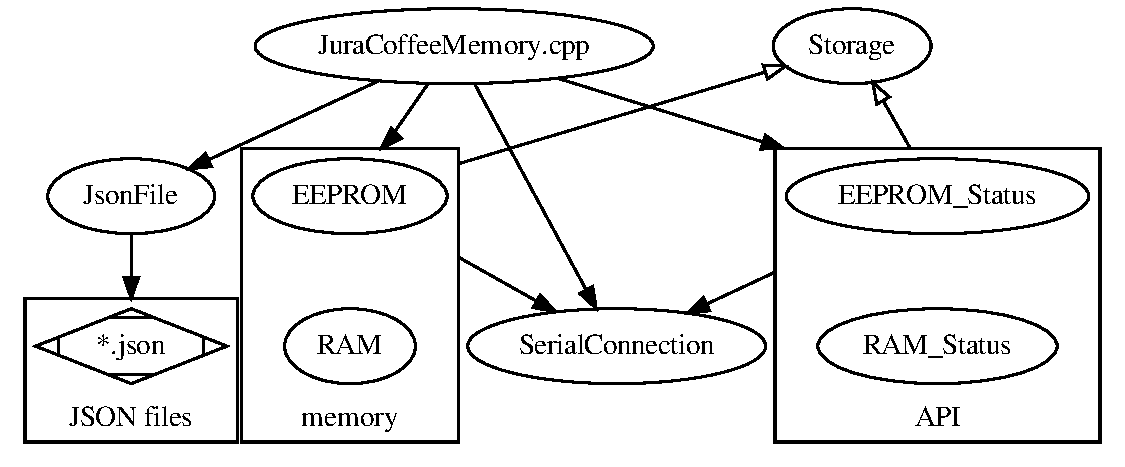
\includegraphics[scale=0.74]{images/chapter_4/class-structure}
    \caption{Schematischer Zusammenhang und Gruppierung der C++ Klassen}
    \label{fig:storage_inherit_graph}
  \end{center}
\end{figure}

\subsubsection{Besonderheiten der technischen Umsetzung / Implementierung}
Die \texttt{EEPROM}- und die \texttt{RAM}-Klasse unterscheiden sich durch die Größenangaben zum Speicher und dem zum Abfragen benötigten Kommando in der entsprechenden \texttt{hpp}-Datei.
Vieles wurde in die gemeinsame Elternklasse \texttt{Storage} ausgegliedert.

Die \texttt{SerialConnection} Klasse setzt das \textit{Singleton-Entwurfsmuster} um\footnote{Die \texttt{JsonFile} Klasse folgt ebenfalls dem Singleton-Entwurfsmuster.}.
Es wird automatisch eine Instanz der Klasse erstellt und ist über eine statische Methode abrufbar.
Dies stellt sicher, dass es nur eine serielle Verbindung zur Zeit gibt.
Darüber hinaus wird beim \texttt{connect()} Methodenaufruf eine Dateisperre auf die serielle Gerätedatei erzeugt.
Dies wiederum garantiert, dass nur eine Prozessinstanz des Programms zur Zeit die Verbindung hält und ungestört bleibt.
Bis zum Aufruf von \texttt{disconnect()} bleibt die Sperre aufrecht erhalten.
Zusätzlich prüft die \texttt{connect()} Methode die Übertragung nach dem Verbindungsaufbau mit dem Testkommando \texttt{TY:} und erwartet von dem Kaffeevollautomaten die eingestellte Antwort \texttt{ty:E1300 CAPU 3\textbackslash r}.
Beim Senden und Empfangen übernehmen die entsprechenden Methoden die Handhabung des Wagenrücklaufs und des Zeilenumbruchs am Ende der Kommandos.
Der Anwender oder Entwickler kann dadurch die Kommandos aus Tabelle~\ref{tbl:kommandos} direkt anwenden.

Die Klassen \texttt{EEPROM\_Status} und \texttt{RAM\_Status} besitzen auch eine Besonderheit.
Die gleich lautende \texttt{scan()} Methode fragt nicht nur die nötigen Speicherstellen ab, sondern vermerkt in dem Vektor \texttt{known\_bytes} ebenfalls deren Position.
Wenn die Methode \texttt{getEntriesEEPROM()} bzw. \texttt{getEntriesRAM()} um weitere Speicherstellen ergänzt wird, ist dadurch sichergestellt, dass auch nur tatsächlich abgefragte Speicherstellen und keine konstanten Nullen zurückgegeben werden.
Andernfalls erhält der Entwickler eine Fehlermeldung.
Weitere Einzelheiten sind in der \texttt{Readme.md} im Projektordner festgehalten.

\section{Weitere kleine Tools}\label{subsec:tools}
Im Unterordner \texttt{./tools/} befinden sich nach dem Aufruf von \texttt{make} drei kleine Programme.

\subsection{Formatieren eines Speicherauszugs}\label{subsec:formate-dump}
Ruft man \texttt{./tools/formate-dump} auf, kann man dem Programm eine Zeichenkette aus $1024$ oder $512$ Hexadezimalzeichen übergeben.
Das Programm erkennt an der Größe \ac{EEPROM} und \ac{RAM} Eingaben und wertet den Speicherauszug um Angaben wie die Speicherposition und Dezimal-/Hexadezimalzahlen Formate auf.

\subsection{Display}
Um den verfügbaren Zeichensatz des Displays in der oberen linken Ecke an der Front des Kaffeevollautomaten zu bestimmen, wurde ein kleines Extraprogramm entwickelt.
Anlass waren Sonderzeichen und die deutschen Umlaute, die sich über die gegebenen Befehle (\texttt{?D0}, \texttt{?D1xxx}, \texttt{?D2xxx}) nicht einfach auf das Display bringen ließen.
Das Programm \texttt{./tools/display} iterierte dafür systematisch über die Zahlen von $0$ bis ungefähr $260$ und gab einen Befehl zum Anzeigen der Dezimalzahl sowie des dazugehörigen \ac{ASCII}-Zeichens an den Kaffeevollautomaten.
Dies umfasst das einfache und erweiterte \ac{ASCII} Alphabet sowie einige weitere Zahlen bzw. Zeichen.
Dabei stellte sich nur ein mittlerer Block des einfachen \ac{ASCII}-Alphabets als interessant heraus, der jetzt eingegrenzt von eben diesem Programm durchlaufen wird.
Ein weiteres Programm namens \texttt{./tools/display-screen-saver} veranschaulicht die damit verbundenen Möglichkeiten.

Die gegebenen Befehle über die serielle Verbindung \texttt{?D0}, \texttt{?D1xxx} und \texttt{?D2xxx} verändern nur den Standardtext "`Kaffee bereit"'.
Andere Texte, wie das Programmmenü oder Warnmeldungen, überlagern den Standardtext mit den einprogrammierten Texten aus den vorhandenen Sprachen.

Möchte man die Ausgaben des ersten Programms nachstellen, ist zu beachten, dass der Kaffeevollautomat eingeschaltet sein muss und auch an die erste Displayzeile ein Ausgabebefehl gegangen sein muss, damit die Ausgabe sichtbar wird.
Das Programm verändert dann die zweite Zeile.
Folgende Befehlseingaben werden empfohlen:
\begin{enumerate}
  \item \texttt{cd JuraCoffeeMemory/}
  \item \texttt{make}
  \item \texttt{./JuraCoffeeMemory}
  \item \texttt{4} (Senden eines Kommandos)
  \item \texttt{AN:01} (Maschine einschalten)
  \item \texttt{?D1xxx} (Etwas Text an die erste Displayzeile)
  \item \texttt{<Strg>+D} (Verlassen des Programms)
  \item \texttt{./tools/display}
\end{enumerate}

\section{Die Webseite}

Die Webseite ist zu sehen in Abbildung~\ref{fig:website}.
Nach ein paar Hinweisen kann im oberen Bereich der einzelne Kaffee sowie die gesamte Maschine konfiguriert werden.
Für jede Kaffeeart ist es möglich, sich seine eigene Konfiguration in einem lokalen Webbrowser-Keks (Cookie) abzuspeichern und komfortabel in den Speicher des Kaffeevollautomaten zu schreiben um sich anschließend einen Kaffee zubereiten zu lassen.
Der Keks kann auch wieder entfernt werden oder sich auf die Standardwerte zurücksetzen lassen.
Prinzipiell kann hierüber der ganze bekannte \ac{EEPROM} überschrieben werden.

Im nächsten Absatz sind Statusinformationen aus dem \ac{RAM} einsehbar.
Einige Meldungen werden am Bild des Kaffeevollautomaten visualisiert.
Der Status kann über \texttt{Refresh} aktualisiert werden.
Einfache "`ja"' oder "`nein"' Meldungen werden durch eine grünes "`on"' oder rotes "`off"' präsentiert.
Informationen, die sich über mehrere Bits erstrecken, werden mit ihrem entsprechenden Zahlenwert dargestellt.

Im letzten Abschnitt befinden sich Zählerstände und Prozent-Anzeigen, die verdeutlichen wie weit es noch bis zur nächsten Warnmeldung, wie Trester leeren, Maschine reinigen oder Filter wechseln, ist.

Wenn am Computer der Mauszeiger auf einer Zahl oder Einstellung zum Finger wird, öffnet sich mit einem Klick ein Fenster, in dem der Wert verändert werden kann.
Nach Möglichkeit werden der Standardwert, der Wert zum Deaktivieren und weitere Hinweis-Texte angeboten.

Unten rechts auf der Seite kann über \texttt{Command} ein Kommando aus der Tabelle~\ref{tbl:kommandos} an den Kaffeevollautomaten abgesetzt werden.
Eine Liste bietet viele Vorschläge mit dazugehörigen Bezeichnungen.
Rechts daneben aktualisiert ein Klick auf \texttt{Refresh} die Statusinformationen aus dem \ac{RAM}.
Ganz rechts in der Ecke kann eine Tour durch die Bedienung der Seite gestartet werden.

\begin{figure}
  \begin{center}
    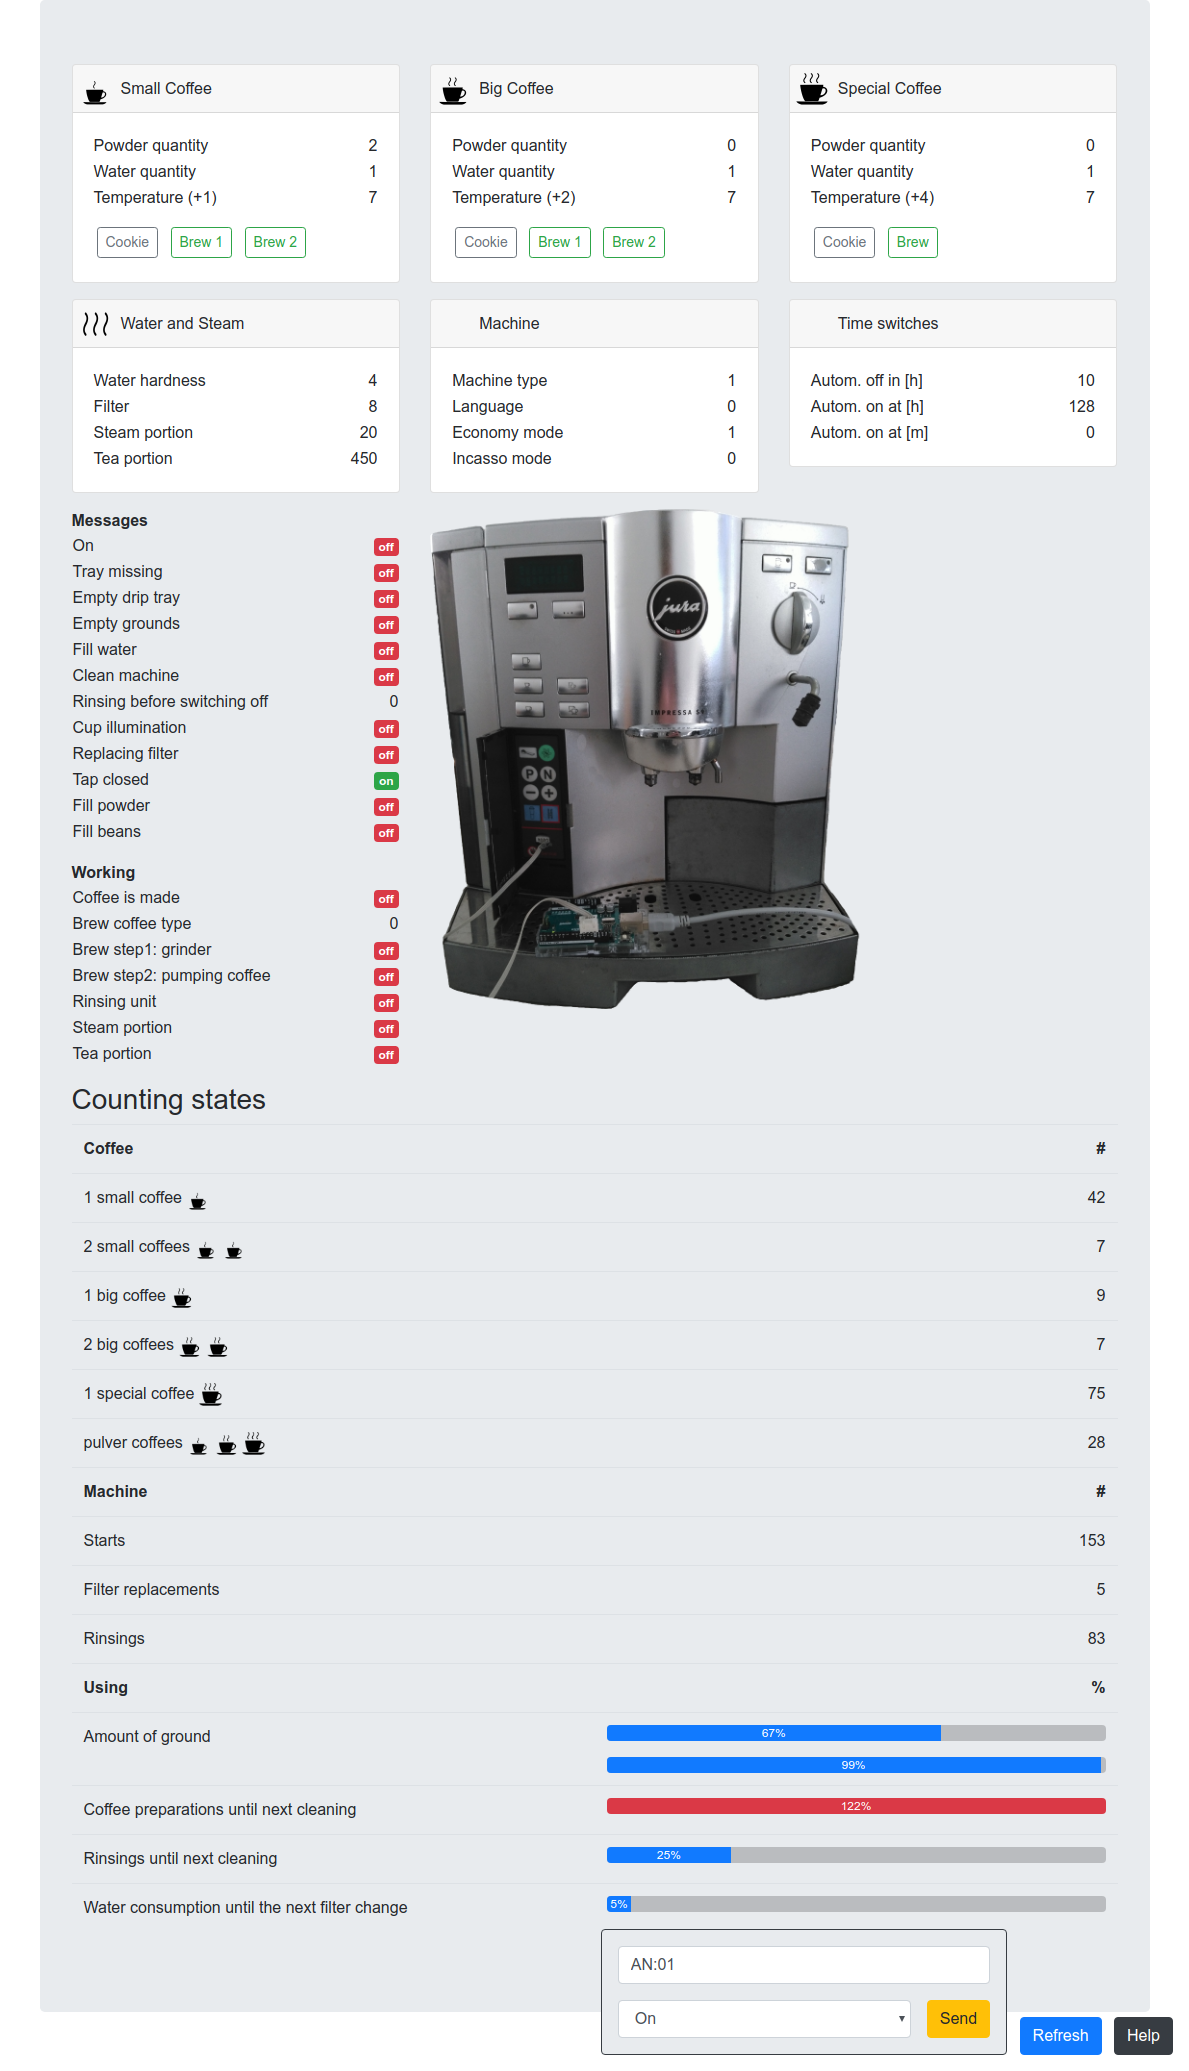
\includegraphics[scale=0.3]{images/chapter_4/Webseite}
    \caption{Webseite zur Kontrolle und Steuerung des Kaffeevollautomaten als Visualisierung der API.}
    \label{fig:website}
  \end{center}
\end{figure}

\subsection{Technische Umsetzung}
Die Webseite befindet sich im Projektunterordner \texttt{./website/}.
Die Datei \texttt{data.php} nimmt Parameter entgegen und ruft damit das C++ Programm mit evtl. Datenübergaben auf.
Die Antwort des C++ Programms wird in einem \ac{JSON}-Objekt verpackt und der Webseite zurück gegeben.
Bei Problemen wird auch die Fehlernummer (der Rückgabewert des Programms) einschließlich der Meldung leicht zugänglich in einem \ac{JSON}-Objekt zurück gegeben.

Die für den Benutzer ersichtliche Webseite besteht primär aus den Dateien \texttt{index.html}, \texttt{script.js} für die Interaktion und \texttt{style.css} für das individuelle Layout.
Weitere eingebundene Dateien sind das Favicon im Unterordner \texttt{favicon/}, Bilder im Unterordner \texttt{img/}, \texttt{intro.min.js} und \texttt{intro.min.css} für die Tour durch die Webseite.
\texttt{offline\_eeprom.json} und \texttt{offline\_ram.json} bieten Beispielwerte für eine Offline-Funktion, in der die Webseite ersichtlich wird, ohne eine Verbindung zu dem Kaffeevollautomaten zu haben.

Das \ac{HTML} Dokument der Webseite besteht aus vielen leeren Inhaltselementen, die im Attribut \texttt{id="..."} Einträge haben, die mit den Bezeichnungen der \ac{JSON} Elemente der Ausgabe von der API des C++ Programms übereinstimmen.
Beim Seitenaufbau wird der \ac{EEPROM} abgefragt.
Wenn die Antwort nach ungefähr 5~Sekunden vorliegt wird der \ac{RAM} abgefragt und anschließend nach ungefähr weiteren 3~Sekunden für jeden \ac{JSON} Eintrag der Wert in das gleichnamige \ac{HTML} Inhaltselement eingetragen.

Eine Ausnahme bildet die Temperatur, die für alle drei Kaffeegrößen gilt, aber im Dokument drei verschiedene ID-Bezeichnungen besitzen muss.
Ebenso ist etwas Handarbeit bei der Ausgabe der Prozent-Anzeigen vonnöten.

Das bei einem Klick aufgehende Fenster zum Bearbeiten von Werten aus dem \ac{EEPROM} arbeitet ebenfalls über die ID-Bezeichnung und entnimmt weitere Informationen aus dem \ac{JSON} Objekt welches zuletzt abgefragt und abgespeichert wurde.
